\documentclass[twoside]{book}

% Packages required by doxygen
\usepackage{fixltx2e}
\usepackage{calc}
\usepackage{doxygen}
\usepackage[export]{adjustbox} % also loads graphicx
\usepackage{graphicx}
\usepackage[utf8]{inputenc}
\usepackage{makeidx}
\usepackage{multicol}
\usepackage{multirow}
\PassOptionsToPackage{warn}{textcomp}
\usepackage{textcomp}
\usepackage[nointegrals]{wasysym}
\usepackage[table]{xcolor}

% Font selection
\usepackage[T1]{fontenc}
\usepackage[scaled=.90]{helvet}
\usepackage{courier}
\usepackage{amssymb}
\usepackage{sectsty}
\renewcommand{\familydefault}{\sfdefault}
\allsectionsfont{%
  \fontseries{bc}\selectfont%
  \color{darkgray}%
}
\renewcommand{\DoxyLabelFont}{%
  \fontseries{bc}\selectfont%
  \color{darkgray}%
}
\newcommand{\+}{\discretionary{\mbox{\scriptsize$\hookleftarrow$}}{}{}}

% Page & text layout
\usepackage{geometry}
\geometry{%
  a4paper,%
  top=2.5cm,%
  bottom=2.5cm,%
  left=2.5cm,%
  right=2.5cm%
}
\tolerance=750
\hfuzz=15pt
\hbadness=750
\setlength{\emergencystretch}{15pt}
\setlength{\parindent}{0cm}
\setlength{\parskip}{3ex plus 2ex minus 2ex}
\makeatletter
\renewcommand{\paragraph}{%
  \@startsection{paragraph}{4}{0ex}{-1.0ex}{1.0ex}{%
    \normalfont\normalsize\bfseries\SS@parafont%
  }%
}
\renewcommand{\subparagraph}{%
  \@startsection{subparagraph}{5}{0ex}{-1.0ex}{1.0ex}{%
    \normalfont\normalsize\bfseries\SS@subparafont%
  }%
}
\makeatother

% Headers & footers
\usepackage{fancyhdr}
\pagestyle{fancyplain}
\fancyhead[LE]{\fancyplain{}{\bfseries\thepage}}
\fancyhead[CE]{\fancyplain{}{}}
\fancyhead[RE]{\fancyplain{}{\bfseries\leftmark}}
\fancyhead[LO]{\fancyplain{}{\bfseries\rightmark}}
\fancyhead[CO]{\fancyplain{}{}}
\fancyhead[RO]{\fancyplain{}{\bfseries\thepage}}
\fancyfoot[LE]{\fancyplain{}{}}
\fancyfoot[CE]{\fancyplain{}{}}
\fancyfoot[RE]{\fancyplain{}{\bfseries\scriptsize Generated by Doxygen }}
\fancyfoot[LO]{\fancyplain{}{\bfseries\scriptsize Generated by Doxygen }}
\fancyfoot[CO]{\fancyplain{}{}}
\fancyfoot[RO]{\fancyplain{}{}}
\renewcommand{\footrulewidth}{0.4pt}
\renewcommand{\chaptermark}[1]{%
  \markboth{#1}{}%
}
\renewcommand{\sectionmark}[1]{%
  \markright{\thesection\ #1}%
}

% Indices & bibliography
\usepackage{natbib}
\usepackage[titles]{tocloft}
\setcounter{tocdepth}{3}
\setcounter{secnumdepth}{5}
\makeindex

% Hyperlinks (required, but should be loaded last)
\usepackage{ifpdf}
\ifpdf
  \usepackage[pdftex,pagebackref=true]{hyperref}
\else
  \usepackage[ps2pdf,pagebackref=true]{hyperref}
\fi
\hypersetup{%
  colorlinks=true,%
  linkcolor=blue,%
  citecolor=blue,%
  unicode%
}

% Custom commands
\newcommand{\clearemptydoublepage}{%
  \newpage{\pagestyle{empty}\cleardoublepage}%
}

\usepackage{caption}
\captionsetup{labelsep=space,justification=centering,font={bf},singlelinecheck=off,skip=4pt,position=top}

%===== C O N T E N T S =====

\begin{document}

% Titlepage & ToC
\hypersetup{pageanchor=false,
             bookmarksnumbered=true,
             pdfencoding=unicode
            }
\pagenumbering{alph}
\begin{titlepage}
\vspace*{7cm}
\begin{center}%
{\Large Jeero }\\
\vspace*{1cm}
{\large Generated by Doxygen 1.8.13}\\
\end{center}
\end{titlepage}
\clearemptydoublepage
\pagenumbering{roman}
\tableofcontents
\clearemptydoublepage
\pagenumbering{arabic}
\hypersetup{pageanchor=true}

%--- Begin generated contents ---
\chapter{Jeero}
\label{index}\hypertarget{index}{}\begin{DoxyAuthor}{Author}
Jeroen Schmit 
\end{DoxyAuthor}
\begin{DoxyVersion}{Version}
1.\+0 
\end{DoxyVersion}
\begin{DoxyCopyright}{Copyright}
G\+NU Public License
\end{DoxyCopyright}
\hypertarget{index_intro}{}\section{Introduction}\label{index_intro}
\hyperlink{namespaceJeero}{Jeero} is a little boy who dreams of going to the theater. He maintains a list of Theaters. His Mother faithfully calls all Theaters and ask them for a Subscription to their list of Shows. He then Works diligently through all the data to put it in one of his beautiful Calendars.

{\itshape \hyperlink{namespaceJeero}{Jeero} also syncs all events and tickets from your ticketing solution with your favourite calendar plugin.} 
\chapter{Namespace Index}
\section{Namespace List}
Here is a list of all documented namespaces with brief descriptions\+:\begin{DoxyCompactList}
\item\contentsline{section}{\hyperlink{namespaceJeero}{Jeero} }{\pageref{namespaceJeero}}{}
\item\contentsline{section}{\hyperlink{namespaceJeero_1_1Admin}{Jeero\textbackslash{}\+Admin} }{\pageref{namespaceJeero_1_1Admin}}{}
\item\contentsline{section}{\hyperlink{namespaceJeero_1_1Calendars}{Jeero\textbackslash{}\+Calendars} }{\pageref{namespaceJeero_1_1Calendars}}{}
\item\contentsline{section}{\hyperlink{namespaceJeero_1_1Db}{Jeero\textbackslash{}\+Db} }{\pageref{namespaceJeero_1_1Db}}{}
\item\contentsline{section}{\hyperlink{namespaceJeero_1_1Mother}{Jeero\textbackslash{}\+Mother} }{\pageref{namespaceJeero_1_1Mother}}{}
\item\contentsline{section}{\hyperlink{namespaceJeero_1_1Subscriptions}{Jeero\textbackslash{}\+Subscriptions} }{\pageref{namespaceJeero_1_1Subscriptions}}{}
\item\contentsline{section}{\hyperlink{namespaceJeero_1_1Theaters}{Jeero\textbackslash{}\+Theaters} }{\pageref{namespaceJeero_1_1Theaters}}{}
\item\contentsline{section}{\hyperlink{namespaceJeero_1_1Work}{Jeero\textbackslash{}\+Work} }{\pageref{namespaceJeero_1_1Work}}{}
\end{DoxyCompactList}

\chapter{Hierarchical Index}
\section{Class Hierarchy}
This inheritance list is sorted roughly, but not completely, alphabetically\+:\begin{DoxyCompactList}
\item \contentsline{section}{Jeero\textbackslash{}Calendars\textbackslash{}Calendar}{\pageref{classJeero_1_1Calendars_1_1Calendar}}{}
\begin{DoxyCompactList}
\item \contentsline{section}{Jeero\textbackslash{}Calendars\textbackslash{}The\+\_\+\+Events\+\_\+\+Calendar}{\pageref{classJeero_1_1Calendars_1_1The__Events__Calendar}}{}
\item \contentsline{section}{Jeero\textbackslash{}Calendars\textbackslash{}The\+\_\+\+Events\+\_\+\+Calendar}{\pageref{classJeero_1_1Calendars_1_1The__Events__Calendar}}{}
\item \contentsline{section}{Jeero\textbackslash{}Calendars\textbackslash{}Theater\+\_\+\+For\+\_\+\+Word\+Press}{\pageref{classJeero_1_1Calendars_1_1Theater__For__WordPress}}{}
\item \contentsline{section}{Jeero\textbackslash{}Calendars\textbackslash{}Theater\+\_\+\+For\+\_\+\+Word\+Press}{\pageref{classJeero_1_1Calendars_1_1Theater__For__WordPress}}{}
\end{DoxyCompactList}
\item \contentsline{section}{Jeero\textbackslash{}Subscriptions\textbackslash{}Subscription}{\pageref{classJeero_1_1Subscriptions_1_1Subscription}}{}
\item \contentsline{section}{Jeero\textbackslash{}Work\textbackslash{}Task}{\pageref{classJeero_1_1Work_1_1Task}}{}
\begin{DoxyCompactList}
\item \contentsline{section}{Jeero\textbackslash{}Work\textbackslash{}Import}{\pageref{classJeero_1_1Work_1_1Import}}{}
\end{DoxyCompactList}
\item \contentsline{section}{Jeero\textbackslash{}Theaters\textbackslash{}Theater}{\pageref{classJeero_1_1Theaters_1_1Theater}}{}
\begin{DoxyCompactList}
\item \contentsline{section}{Jeero\textbackslash{}Theaters\textbackslash{}Veezi}{\pageref{classJeero_1_1Theaters_1_1Veezi}}{}
\item \contentsline{section}{Jeero\textbackslash{}Theaters\textbackslash{}Veezi}{\pageref{classJeero_1_1Theaters_1_1Veezi}}{}
\end{DoxyCompactList}
\end{DoxyCompactList}

\chapter{Class Index}
\section{Class List}
Here are the classes, structs, unions and interfaces with brief descriptions\+:\begin{DoxyCompactList}
\item\contentsline{section}{\hyperlink{classJeero_1_1Calendars_1_1Calendar}{Jeero\textbackslash{}\+Calendars\textbackslash{}\+Calendar} }{\pageref{classJeero_1_1Calendars_1_1Calendar}}{}
\item\contentsline{section}{\hyperlink{classJeero_1_1Work_1_1Import}{Jeero\textbackslash{}\+Work\textbackslash{}\+Import} }{\pageref{classJeero_1_1Work_1_1Import}}{}
\item\contentsline{section}{\hyperlink{classJeero_1_1Subscriptions_1_1Subscription}{Jeero\textbackslash{}\+Subscriptions\textbackslash{}\+Subscription} }{\pageref{classJeero_1_1Subscriptions_1_1Subscription}}{}
\item\contentsline{section}{\hyperlink{classJeero_1_1Work_1_1Task}{Jeero\textbackslash{}\+Work\textbackslash{}\+Task} }{\pageref{classJeero_1_1Work_1_1Task}}{}
\item\contentsline{section}{\hyperlink{classJeero_1_1Calendars_1_1The__Events__Calendar}{Jeero\textbackslash{}\+Calendars\textbackslash{}\+The\+\_\+\+Events\+\_\+\+Calendar} }{\pageref{classJeero_1_1Calendars_1_1The__Events__Calendar}}{}
\item\contentsline{section}{\hyperlink{classJeero_1_1Theaters_1_1Theater}{Jeero\textbackslash{}\+Theaters\textbackslash{}\+Theater} }{\pageref{classJeero_1_1Theaters_1_1Theater}}{}
\item\contentsline{section}{\hyperlink{classJeero_1_1Calendars_1_1Theater__For__WordPress}{Jeero\textbackslash{}\+Calendars\textbackslash{}\+Theater\+\_\+\+For\+\_\+\+Word\+Press} }{\pageref{classJeero_1_1Calendars_1_1Theater__For__WordPress}}{}
\item\contentsline{section}{\hyperlink{classJeero_1_1Theaters_1_1Veezi}{Jeero\textbackslash{}\+Theaters\textbackslash{}\+Veezi} }{\pageref{classJeero_1_1Theaters_1_1Veezi}}{}
\end{DoxyCompactList}

\chapter{Namespace Documentation}
\hypertarget{namespaceJeero}{}\section{Jeero Namespace Reference}
\label{namespaceJeero}\index{Jeero@{Jeero}}
\subsection*{Namespaces}
\begin{DoxyCompactItemize}
\item 
 \hyperlink{namespaceJeero_1_1Admin}{Admin}
\item 
 \hyperlink{namespaceJeero_1_1Calendars}{Calendars}
\item 
 \hyperlink{namespaceJeero_1_1Db}{Db}
\item 
 \hyperlink{namespaceJeero_1_1Mother}{Mother}
\item 
 \hyperlink{namespaceJeero_1_1Subscriptions}{Subscriptions}
\item 
 \hyperlink{namespaceJeero_1_1Theaters}{Theaters}
\item 
 \hyperlink{namespaceJeero_1_1Work}{Work}
\end{DoxyCompactItemize}


\subsection{Detailed Description}
Hi! I am \hyperlink{namespaceJeero}{Jeero}. 
\hypertarget{namespaceJeero_1_1Admin}{}\section{Jeero\textbackslash{}Admin Namespace Reference}
\label{namespaceJeero_1_1Admin}\index{Jeero\textbackslash{}\+Admin@{Jeero\textbackslash{}\+Admin}}
\subsection*{Functions}
\begin{DoxyCompactItemize}
\item 
\mbox{\Hypertarget{namespaceJeero_1_1Admin_ab3431ee74882551b0d3e0c4b35848b7a}\label{namespaceJeero_1_1Admin_ab3431ee74882551b0d3e0c4b35848b7a}} 
{\bfseries add\+\_\+menu\+\_\+item} ()
\item 
\mbox{\Hypertarget{namespaceJeero_1_1Admin_aa3fc419a7f4ccf70acc767fde777b635}\label{namespaceJeero_1_1Admin_aa3fc419a7f4ccf70acc767fde777b635}} 
{\bfseries add\+\_\+admin\+\_\+screen} ()
\end{DoxyCompactItemize}


\subsection{Detailed Description}
Handles all \hyperlink{namespaceJeero}{Jeero} admin screens. 
\hypertarget{namespaceJeero_1_1Calendars}{}\section{Jeero\textbackslash{}Calendars Namespace Reference}
\label{namespaceJeero_1_1Calendars}\index{Jeero\textbackslash{}\+Calendars@{Jeero\textbackslash{}\+Calendars}}
\subsection*{Classes}
\begin{DoxyCompactItemize}
\item 
class \hyperlink{classJeero_1_1Calendars_1_1Calendar}{Calendar}
\item 
class \hyperlink{classJeero_1_1Calendars_1_1The__Events__Calendar}{The\+\_\+\+Events\+\_\+\+Calendar}
\item 
class \hyperlink{classJeero_1_1Calendars_1_1Theater__For__WordPress}{Theater\+\_\+\+For\+\_\+\+Word\+Press}
\end{DoxyCompactItemize}


\subsection{Detailed Description}
\hyperlink{namespaceJeero}{Jeero} add all Shows to his \hyperlink{classJeero_1_1Calendars_1_1Calendar}{Calendar}. 
\hypertarget{namespaceJeero_1_1Db}{}\section{Jeero\textbackslash{}Db Namespace Reference}
\label{namespaceJeero_1_1Db}\index{Jeero\textbackslash{}\+Db@{Jeero\textbackslash{}\+Db}}
\subsection*{Functions}
\begin{DoxyCompactItemize}
\item 
\mbox{\Hypertarget{namespaceJeero_1_1Db_a561030bb75e2ac27c9203ac49ed9e267}\label{namespaceJeero_1_1Db_a561030bb75e2ac27c9203ac49ed9e267}} 
{\bfseries get\+\_\+subscription} ( \$ID)
\item 
\mbox{\Hypertarget{namespaceJeero_1_1Db_a489bf14547c01ad7a7a4d6980653d19f}\label{namespaceJeero_1_1Db_a489bf14547c01ad7a7a4d6980653d19f}} 
{\bfseries save\+\_\+subscription} ( \$ID, \$data)
\item 
\hyperlink{namespaceJeero_1_1Db_aeeae82925ec06323d8a39bad5f79113e}{upgrade\+\_\+100} ()
\item 
\hyperlink{namespaceJeero_1_1Db_aa6128a08cd67244aa44fd408b532cd06}{upgrade} ()
\end{DoxyCompactItemize}


\subsection{Detailed Description}
Handles all communication with the custom \hyperlink{namespaceJeero}{Jeero} tables in the database. 

\subsection{Function Documentation}
\mbox{\Hypertarget{namespaceJeero_1_1Db_aa6128a08cd67244aa44fd408b532cd06}\label{namespaceJeero_1_1Db_aa6128a08cd67244aa44fd408b532cd06}} 
\index{Jeero\+::\+Db@{Jeero\+::\+Db}!upgrade@{upgrade}}
\index{upgrade@{upgrade}!Jeero\+::\+Db@{Jeero\+::\+Db}}
\subsubsection{\texorpdfstring{upgrade()}{upgrade()}}
{\footnotesize\ttfamily Jeero\textbackslash{}\+Db\textbackslash{}upgrade (\begin{DoxyParamCaption}{ }\end{DoxyParamCaption})}

Upgrades the \hyperlink{namespaceJeero}{Jeero} tables to the most recente version.

\begin{DoxyReturn}{Returns}
void 
\end{DoxyReturn}
\mbox{\Hypertarget{namespaceJeero_1_1Db_aeeae82925ec06323d8a39bad5f79113e}\label{namespaceJeero_1_1Db_aeeae82925ec06323d8a39bad5f79113e}} 
\index{Jeero\+::\+Db@{Jeero\+::\+Db}!upgrade\+\_\+100@{upgrade\+\_\+100}}
\index{upgrade\+\_\+100@{upgrade\+\_\+100}!Jeero\+::\+Db@{Jeero\+::\+Db}}
\subsubsection{\texorpdfstring{upgrade\+\_\+100()}{upgrade\_100()}}
{\footnotesize\ttfamily Jeero\textbackslash{}\+Db\textbackslash{}upgrade\+\_\+100 (\begin{DoxyParamCaption}{ }\end{DoxyParamCaption})}

Upgrades the \hyperlink{namespaceJeero}{Jeero} tables to version 1.\+0.

\begin{DoxySince}{Since}
1.\+0 
\end{DoxySince}
\begin{DoxyReturn}{Returns}
bool 
\end{DoxyReturn}

\hypertarget{namespaceJeero_1_1Mother}{}\section{Jeero\textbackslash{}Mother Namespace Reference}
\label{namespaceJeero_1_1Mother}\index{Jeero\textbackslash{}\+Mother@{Jeero\textbackslash{}\+Mother}}
\subsection*{Functions}
\begin{DoxyCompactItemize}
\item 
\hyperlink{namespaceJeero_1_1Mother_ad8898f9d86248f6c1999c6bed607a939}{check\+\_\+status} (\hyperlink{classJeero_1_1Subscriptions_1_1Subscription}{Subscription} \$subscription)
\item 
\hyperlink{namespaceJeero_1_1Mother_af3a7a0928f56dae13cf5380a264e8a91}{get\+\_\+subscriptions} ()
\item 
\hyperlink{namespaceJeero_1_1Mother_a379b77ef6336a987a5359b5b28212259}{subscribe\+\_\+me} ( \$settings=array())
\item 
\mbox{\Hypertarget{namespaceJeero_1_1Mother_a8e51738b255a4f47b25aab29166d93c5}\label{namespaceJeero_1_1Mother_a8e51738b255a4f47b25aab29166d93c5}} 
{\bfseries get} ( \$endpoint, \$data=array())
\item 
\mbox{\Hypertarget{namespaceJeero_1_1Mother_a481c663ee8111e8d35e10214eecd2725}\label{namespaceJeero_1_1Mother_a481c663ee8111e8d35e10214eecd2725}} 
{\bfseries post} ( \$endpoint, \$data=array())
\end{DoxyCompactItemize}
\subsection*{Variables}
\begin{DoxyCompactItemize}
\item 
\mbox{\Hypertarget{namespaceJeero_1_1Mother_a66d3570f9eaddc0483d4623549d265f4}\label{namespaceJeero_1_1Mother_a66d3570f9eaddc0483d4623549d265f4}} 
const {\bfseries B\+A\+S\+E\+\_\+\+U\+RL} = \textquotesingle{}https\+://mother.\+jeero.\+ooo\textquotesingle{}
\end{DoxyCompactItemize}


\subsection{Detailed Description}
Sends \hyperlink{namespaceJeero_1_1Mother}{Mother} out to visit \hyperlink{namespaceJeero_1_1Theaters}{Theaters}. 

\subsection{Function Documentation}
\mbox{\Hypertarget{namespaceJeero_1_1Mother_ad8898f9d86248f6c1999c6bed607a939}\label{namespaceJeero_1_1Mother_ad8898f9d86248f6c1999c6bed607a939}} 
\index{Jeero\+::\+Mother@{Jeero\+::\+Mother}!check\+\_\+status@{check\+\_\+status}}
\index{check\+\_\+status@{check\+\_\+status}!Jeero\+::\+Mother@{Jeero\+::\+Mother}}
\subsubsection{\texorpdfstring{check\+\_\+status()}{check\_status()}}
{\footnotesize\ttfamily Jeero\textbackslash{}\+Mother\textbackslash{}check\+\_\+status (\begin{DoxyParamCaption}\item[{\hyperlink{classJeero_1_1Subscriptions_1_1Subscription}{Subscription}}]{\$subscription }\end{DoxyParamCaption})}

Asks \hyperlink{namespaceJeero_1_1Mother}{Mother} to remind a Theater about a Subscription.

\begin{DoxySince}{Since}
1.\+0 
\end{DoxySince}

\begin{DoxyParams}[1]{Parameters}
Subscription & {\em \$subscription} & The Subscription. \\
\hline
\end{DoxyParams}
\begin{DoxyReturn}{Returns}
boolean$\vert$\+W\+P\+\_\+\+Error $<$true$>$ if successful. An error if there was a problem. 
\end{DoxyReturn}
\mbox{\Hypertarget{namespaceJeero_1_1Mother_af3a7a0928f56dae13cf5380a264e8a91}\label{namespaceJeero_1_1Mother_af3a7a0928f56dae13cf5380a264e8a91}} 
\index{Jeero\+::\+Mother@{Jeero\+::\+Mother}!get\+\_\+subscriptions@{get\+\_\+subscriptions}}
\index{get\+\_\+subscriptions@{get\+\_\+subscriptions}!Jeero\+::\+Mother@{Jeero\+::\+Mother}}
\subsubsection{\texorpdfstring{get\+\_\+subscriptions()}{get\_subscriptions()}}
{\footnotesize\ttfamily Jeero\textbackslash{}\+Mother\textbackslash{}get\+\_\+subscriptions (\begin{DoxyParamCaption}{ }\end{DoxyParamCaption})}

Asks \hyperlink{namespaceJeero_1_1Mother}{Mother} for a list of all \hyperlink{namespaceJeero_1_1Subscriptions}{Subscriptions}.

\begin{DoxyReturn}{Returns}
Subscription\mbox{[}\mbox{]}$\vert$\+W\+P\+\_\+\+Error All \hyperlink{namespaceJeero_1_1Subscriptions}{Subscriptions} or an error if there is a problem. 
\end{DoxyReturn}
\mbox{\Hypertarget{namespaceJeero_1_1Mother_a379b77ef6336a987a5359b5b28212259}\label{namespaceJeero_1_1Mother_a379b77ef6336a987a5359b5b28212259}} 
\index{Jeero\+::\+Mother@{Jeero\+::\+Mother}!subscribe\+\_\+me@{subscribe\+\_\+me}}
\index{subscribe\+\_\+me@{subscribe\+\_\+me}!Jeero\+::\+Mother@{Jeero\+::\+Mother}}
\subsubsection{\texorpdfstring{subscribe\+\_\+me()}{subscribe\_me()}}
{\footnotesize\ttfamily Jeero\textbackslash{}\+Mother\textbackslash{}subscribe\+\_\+me (\begin{DoxyParamCaption}\item[{}]{\$settings = {\ttfamily array()} }\end{DoxyParamCaption})}

Asks \hyperlink{namespaceJeero_1_1Mother}{Mother} to set up a new Subscription with a Theater.

\begin{DoxyReturn}{Returns}
Subscription$\vert$\+W\+P\+\_\+\+Error The new Subscription or an error if there was a problem. 
\end{DoxyReturn}

\hypertarget{namespaceJeero_1_1Subscriptions}{}\section{Jeero\textbackslash{}Subscriptions Namespace Reference}
\label{namespaceJeero_1_1Subscriptions}\index{Jeero\textbackslash{}\+Subscriptions@{Jeero\textbackslash{}\+Subscriptions}}
\subsection*{Classes}
\begin{DoxyCompactItemize}
\item 
class \hyperlink{classJeero_1_1Subscriptions_1_1Subscription}{Subscription}
\end{DoxyCompactItemize}
\subsection*{Functions}
\begin{DoxyCompactItemize}
\item 
\hyperlink{namespaceJeero_1_1Subscriptions_a7fefeb0c9fc00b9b47bd9da69da6ecbd}{add\+\_\+subscription} ()
\item 
\hyperlink{namespaceJeero_1_1Subscriptions_af143e8607705a82067cfe4082cf5f3a5}{get\+\_\+subscriptions} ()
\item 
\hyperlink{namespaceJeero_1_1Subscriptions_a02cb69ca8b573c4397759a6ddde6af28}{update\+\_\+subscription} (\hyperlink{classJeero_1_1Subscriptions_1_1Subscription}{Subscription} \$subscription, array \$settings)
\item 
\hyperlink{namespaceJeero_1_1Subscriptions_a9d1e85f0c5a276290e41bc794ae9da66}{cancel\+\_\+subscription} (\hyperlink{classJeero_1_1Subscriptions_1_1Subscription}{Subscription} \$subscription)
\end{DoxyCompactItemize}
\subsection*{Variables}
\begin{DoxyCompactItemize}
\item 
\mbox{\Hypertarget{namespaceJeero_1_1Subscriptions_ab76755fd13084faaeeeb80488e71a86f}\label{namespaceJeero_1_1Subscriptions_ab76755fd13084faaeeeb80488e71a86f}} 
const {\bfseries S\+U\+B\+S\+C\+R\+I\+P\+T\+I\+O\+N\+S\+\_\+\+S\+E\+T\+T\+I\+N\+G\+S\+\_\+\+K\+EY} = \textquotesingle{}Jeero/Subscriptions/Settings\textquotesingle{}
\end{DoxyCompactItemize}


\subsection{Detailed Description}
Manages all of \hyperlink{namespaceJeero}{Jeero}\textquotesingle{}s \hyperlink{namespaceJeero_1_1Subscriptions}{Subscriptions}. 

\subsection{Function Documentation}
\mbox{\Hypertarget{namespaceJeero_1_1Subscriptions_a7fefeb0c9fc00b9b47bd9da69da6ecbd}\label{namespaceJeero_1_1Subscriptions_a7fefeb0c9fc00b9b47bd9da69da6ecbd}} 
\index{Jeero\+::\+Subscriptions@{Jeero\+::\+Subscriptions}!add\+\_\+subscription@{add\+\_\+subscription}}
\index{add\+\_\+subscription@{add\+\_\+subscription}!Jeero\+::\+Subscriptions@{Jeero\+::\+Subscriptions}}
\subsubsection{\texorpdfstring{add\+\_\+subscription()}{add\_subscription()}}
{\footnotesize\ttfamily Jeero\textbackslash{}\+Subscriptions\textbackslash{}add\+\_\+subscription (\begin{DoxyParamCaption}{ }\end{DoxyParamCaption})}

Adds a \hyperlink{classJeero_1_1Subscriptions_1_1Subscription}{Subscription}.

\begin{DoxyReturn}{Returns}
\hyperlink{classJeero_1_1Subscriptions_1_1Subscription}{Subscription} The new \hyperlink{classJeero_1_1Subscriptions_1_1Subscription}{Subscription}. 
\end{DoxyReturn}
\mbox{\Hypertarget{namespaceJeero_1_1Subscriptions_a9d1e85f0c5a276290e41bc794ae9da66}\label{namespaceJeero_1_1Subscriptions_a9d1e85f0c5a276290e41bc794ae9da66}} 
\index{Jeero\+::\+Subscriptions@{Jeero\+::\+Subscriptions}!cancel\+\_\+subscription@{cancel\+\_\+subscription}}
\index{cancel\+\_\+subscription@{cancel\+\_\+subscription}!Jeero\+::\+Subscriptions@{Jeero\+::\+Subscriptions}}
\subsubsection{\texorpdfstring{cancel\+\_\+subscription()}{cancel\_subscription()}}
{\footnotesize\ttfamily Jeero\textbackslash{}\+Subscriptions\textbackslash{}cancel\+\_\+subscription (\begin{DoxyParamCaption}\item[{\hyperlink{classJeero_1_1Subscriptions_1_1Subscription}{Subscription}}]{\$subscription }\end{DoxyParamCaption})}

Cancels a \hyperlink{classJeero_1_1Subscriptions_1_1Subscription}{Subscription}.


\begin{DoxyParams}[1]{Parameters}
\hyperlink{classJeero_1_1Subscriptions_1_1Subscription}{Subscription} & {\em \$subscription} & \\
\hline
\end{DoxyParams}
\begin{DoxyReturn}{Returns}
void 
\end{DoxyReturn}
\mbox{\Hypertarget{namespaceJeero_1_1Subscriptions_af143e8607705a82067cfe4082cf5f3a5}\label{namespaceJeero_1_1Subscriptions_af143e8607705a82067cfe4082cf5f3a5}} 
\index{Jeero\+::\+Subscriptions@{Jeero\+::\+Subscriptions}!get\+\_\+subscriptions@{get\+\_\+subscriptions}}
\index{get\+\_\+subscriptions@{get\+\_\+subscriptions}!Jeero\+::\+Subscriptions@{Jeero\+::\+Subscriptions}}
\subsubsection{\texorpdfstring{get\+\_\+subscriptions()}{get\_subscriptions()}}
{\footnotesize\ttfamily Jeero\textbackslash{}\+Subscriptions\textbackslash{}get\+\_\+subscriptions (\begin{DoxyParamCaption}{ }\end{DoxyParamCaption})}

Gets all of \hyperlink{namespaceJeero}{Jeero}\textquotesingle{}s \hyperlink{namespaceJeero_1_1Subscriptions}{Subscriptions}.

\begin{DoxyReturn}{Returns}
\hyperlink{classJeero_1_1Subscriptions_1_1Subscription}{Subscription}\mbox{[}\mbox{]} An array containing all of \hyperlink{namespaceJeero}{Jeero}\textquotesingle{}s \hyperlink{namespaceJeero_1_1Subscriptions}{Subscriptions}. 
\end{DoxyReturn}
\mbox{\Hypertarget{namespaceJeero_1_1Subscriptions_a02cb69ca8b573c4397759a6ddde6af28}\label{namespaceJeero_1_1Subscriptions_a02cb69ca8b573c4397759a6ddde6af28}} 
\index{Jeero\+::\+Subscriptions@{Jeero\+::\+Subscriptions}!update\+\_\+subscription@{update\+\_\+subscription}}
\index{update\+\_\+subscription@{update\+\_\+subscription}!Jeero\+::\+Subscriptions@{Jeero\+::\+Subscriptions}}
\subsubsection{\texorpdfstring{update\+\_\+subscription()}{update\_subscription()}}
{\footnotesize\ttfamily Jeero\textbackslash{}\+Subscriptions\textbackslash{}update\+\_\+subscription (\begin{DoxyParamCaption}\item[{\hyperlink{classJeero_1_1Subscriptions_1_1Subscription}{Subscription}}]{\$subscription,  }\item[{array}]{\$settings }\end{DoxyParamCaption})}

Updates the settings of a \hyperlink{classJeero_1_1Subscriptions_1_1Subscription}{Subscription}.


\begin{DoxyParams}[1]{Parameters}
\hyperlink{classJeero_1_1Subscriptions_1_1Subscription}{Subscription} & {\em \$subscription} & The \hyperlink{classJeero_1_1Subscriptions_1_1Subscription}{Subscription}. \\
\hline
array & {\em \$settings} & The new settings.\\
\hline
\end{DoxyParams}
\begin{DoxyReturn}{Returns}
\hyperlink{classJeero_1_1Subscriptions_1_1Subscription}{Subscription} The updated \hyperlink{classJeero_1_1Subscriptions_1_1Subscription}{Subscription}. 
\end{DoxyReturn}

\hypertarget{namespaceJeero_1_1Theaters}{}\section{Jeero\textbackslash{}Theaters Namespace Reference}
\label{namespaceJeero_1_1Theaters}\index{Jeero\textbackslash{}\+Theaters@{Jeero\textbackslash{}\+Theaters}}
\subsection*{Classes}
\begin{DoxyCompactItemize}
\item 
class \hyperlink{classJeero_1_1Theaters_1_1Theater}{Theater}
\item 
class \hyperlink{classJeero_1_1Theaters_1_1Veezi}{Veezi}
\end{DoxyCompactItemize}


\subsection{Detailed Description}
Manages all \hyperlink{namespaceJeero_1_1Theaters}{Theaters} on \hyperlink{namespaceJeero_1_1Mother}{Mother}\textquotesingle{}s list. 
\hypertarget{namespaceJeero_1_1Work}{}\section{Jeero\textbackslash{}Work Namespace Reference}
\label{namespaceJeero_1_1Work}\index{Jeero\textbackslash{}\+Work@{Jeero\textbackslash{}\+Work}}
\subsection*{Classes}
\begin{DoxyCompactItemize}
\item 
class \hyperlink{classJeero_1_1Work_1_1Import}{Import}
\item 
class \hyperlink{classJeero_1_1Work_1_1Task}{Task}
\end{DoxyCompactItemize}


\subsection{Detailed Description}
Handles all the work that \hyperlink{namespaceJeero}{Jeero} still has to do. 
\chapter{Class Documentation}
\hypertarget{classJeero_1_1Calendars_1_1Calendar}{}\section{Jeero\textbackslash{}Calendars\textbackslash{}Calendar Class Reference}
\label{classJeero_1_1Calendars_1_1Calendar}\index{Jeero\textbackslash{}\+Calendars\textbackslash{}\+Calendar@{Jeero\textbackslash{}\+Calendars\textbackslash{}\+Calendar}}


Inheritance diagram for Jeero\textbackslash{}Calendars\textbackslash{}Calendar\+:\nopagebreak
\begin{figure}[H]
\begin{center}
\leavevmode
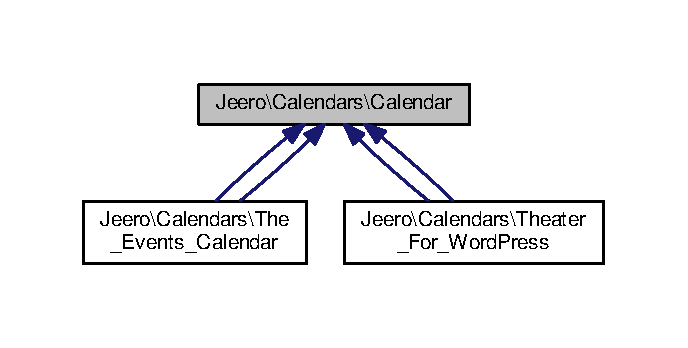
\includegraphics[width=330pt]{classJeero_1_1Calendars_1_1Calendar__inherit__graph}
\end{center}
\end{figure}


The documentation for this class was generated from the following file\+:\begin{DoxyCompactItemize}
\item 
Calendars/Calendar.\+php\end{DoxyCompactItemize}

\hypertarget{classJeero_1_1Work_1_1Import}{}\section{Jeero\textbackslash{}Work\textbackslash{}Import Class Reference}
\label{classJeero_1_1Work_1_1Import}\index{Jeero\textbackslash{}\+Work\textbackslash{}\+Import@{Jeero\textbackslash{}\+Work\textbackslash{}\+Import}}


Inheritance diagram for Jeero\textbackslash{}Work\textbackslash{}Import\+:\nopagebreak
\begin{figure}[H]
\begin{center}
\leavevmode
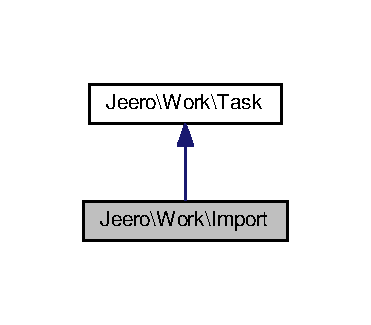
\includegraphics[width=178pt]{classJeero_1_1Work_1_1Import__inherit__graph}
\end{center}
\end{figure}


Collaboration diagram for Jeero\textbackslash{}Work\textbackslash{}Import\+:\nopagebreak
\begin{figure}[H]
\begin{center}
\leavevmode
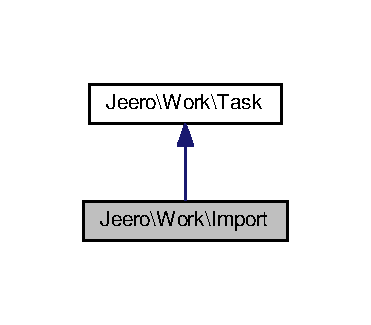
\includegraphics[width=178pt]{classJeero_1_1Work_1_1Import__coll__graph}
\end{center}
\end{figure}


The documentation for this class was generated from the following file\+:\begin{DoxyCompactItemize}
\item 
Work/Import.\+php\end{DoxyCompactItemize}

\hypertarget{classJeero_1_1Subscriptions_1_1Subscription}{}\section{Jeero\textbackslash{}Subscriptions\textbackslash{}Subscription Class Reference}
\label{classJeero_1_1Subscriptions_1_1Subscription}\index{Jeero\textbackslash{}\+Subscriptions\textbackslash{}\+Subscription@{Jeero\textbackslash{}\+Subscriptions\textbackslash{}\+Subscription}}
\subsection*{Public Member Functions}
\begin{DoxyCompactItemize}
\item 
\mbox{\Hypertarget{classJeero_1_1Subscriptions_1_1Subscription_add02e9200cef0f2597062722a7d6af8c}\label{classJeero_1_1Subscriptions_1_1Subscription_add02e9200cef0f2597062722a7d6af8c}} 
{\bfseries \+\_\+\+\_\+construct} ( \$ID)
\item 
\mbox{\Hypertarget{classJeero_1_1Subscriptions_1_1Subscription_a34e23235e49be695c2237f5e1ed45f10}\label{classJeero_1_1Subscriptions_1_1Subscription_a34e23235e49be695c2237f5e1ed45f10}} 
{\bfseries get} ( \$key)
\item 
\mbox{\Hypertarget{classJeero_1_1Subscriptions_1_1Subscription_a131d71552c91f1eb7cb79d2557fb7406}\label{classJeero_1_1Subscriptions_1_1Subscription_a131d71552c91f1eb7cb79d2557fb7406}} 
{\bfseries load} ()
\item 
\mbox{\Hypertarget{classJeero_1_1Subscriptions_1_1Subscription_aba96547151a8c16a7bb5eb2384fea405}\label{classJeero_1_1Subscriptions_1_1Subscription_aba96547151a8c16a7bb5eb2384fea405}} 
{\bfseries set} ( \$key, \$value)
\item 
\mbox{\Hypertarget{classJeero_1_1Subscriptions_1_1Subscription_ae20551c7756dca165baeb6f817729202}\label{classJeero_1_1Subscriptions_1_1Subscription_ae20551c7756dca165baeb6f817729202}} 
{\bfseries save} ()
\end{DoxyCompactItemize}
\subsection*{Public Attributes}
\begin{DoxyCompactItemize}
\item 
\hyperlink{classJeero_1_1Subscriptions_1_1Subscription_a11b976caf4ebbb66d14a4b061ab50245}{\$\+ID}
\item 
\mbox{\Hypertarget{classJeero_1_1Subscriptions_1_1Subscription_a208b09662fbde0228de346e5fd81c260}\label{classJeero_1_1Subscriptions_1_1Subscription_a208b09662fbde0228de346e5fd81c260}} 
{\bfseries \$fields} = array()
\item 
\mbox{\Hypertarget{classJeero_1_1Subscriptions_1_1Subscription_aa87c6f263b1cf17a4df400a5d85cde11}\label{classJeero_1_1Subscriptions_1_1Subscription_aa87c6f263b1cf17a4df400a5d85cde11}} 
{\bfseries \$next\+\_\+update}
\item 
\hyperlink{classJeero_1_1Subscriptions_1_1Subscription_a179357f2a603a38178d60b2018428500}{\$settings} = array()
\item 
\hyperlink{classJeero_1_1Subscriptions_1_1Subscription_af8b68d458d86bc8c8c9f8abe1135eaee}{\$status}
\end{DoxyCompactItemize}


\subsection{Detailed Description}
\hyperlink{classJeero_1_1Subscriptions_1_1Subscription}{Subscription} class. 

\subsection{Member Data Documentation}
\mbox{\Hypertarget{classJeero_1_1Subscriptions_1_1Subscription_a11b976caf4ebbb66d14a4b061ab50245}\label{classJeero_1_1Subscriptions_1_1Subscription_a11b976caf4ebbb66d14a4b061ab50245}} 
\index{Jeero\+::\+Subscriptions\+::\+Subscription@{Jeero\+::\+Subscriptions\+::\+Subscription}!\$\+ID@{\$\+ID}}
\index{\$\+ID@{\$\+ID}!Jeero\+::\+Subscriptions\+::\+Subscription@{Jeero\+::\+Subscriptions\+::\+Subscription}}
\subsubsection{\texorpdfstring{\$\+ID}{$ID}}
{\footnotesize\ttfamily string Jeero\textbackslash{}\+Subscriptions\textbackslash{}\+Subscription\+::\$\+ID}

The ID of this \hyperlink{classJeero_1_1Subscriptions_1_1Subscription}{Subscription}.

\begin{DoxySince}{Since}
1.\+0 
\end{DoxySince}
\mbox{\Hypertarget{classJeero_1_1Subscriptions_1_1Subscription_a179357f2a603a38178d60b2018428500}\label{classJeero_1_1Subscriptions_1_1Subscription_a179357f2a603a38178d60b2018428500}} 
\index{Jeero\+::\+Subscriptions\+::\+Subscription@{Jeero\+::\+Subscriptions\+::\+Subscription}!\$settings@{\$settings}}
\index{\$settings@{\$settings}!Jeero\+::\+Subscriptions\+::\+Subscription@{Jeero\+::\+Subscriptions\+::\+Subscription}}
\subsubsection{\texorpdfstring{\$settings}{$settings}}
{\footnotesize\ttfamily array Jeero\textbackslash{}\+Subscriptions\textbackslash{}\+Subscription\+::\$settings = array()}

The settings of this \hyperlink{classJeero_1_1Subscriptions_1_1Subscription}{Subscription}.

\begin{DoxySince}{Since}
1.\+0 
\end{DoxySince}
\mbox{\Hypertarget{classJeero_1_1Subscriptions_1_1Subscription_af8b68d458d86bc8c8c9f8abe1135eaee}\label{classJeero_1_1Subscriptions_1_1Subscription_af8b68d458d86bc8c8c9f8abe1135eaee}} 
\index{Jeero\+::\+Subscriptions\+::\+Subscription@{Jeero\+::\+Subscriptions\+::\+Subscription}!\$status@{\$status}}
\index{\$status@{\$status}!Jeero\+::\+Subscriptions\+::\+Subscription@{Jeero\+::\+Subscriptions\+::\+Subscription}}
\subsubsection{\texorpdfstring{\$status}{$status}}
{\footnotesize\ttfamily string Jeero\textbackslash{}\+Subscriptions\textbackslash{}\+Subscription\+::\$status}

The status of this \hyperlink{classJeero_1_1Subscriptions_1_1Subscription}{Subscription}.

\begin{DoxySince}{Since}
1.\+0 
\end{DoxySince}


The documentation for this class was generated from the following file\+:\begin{DoxyCompactItemize}
\item 
Subscriptions/Subscription.\+php\end{DoxyCompactItemize}

\hypertarget{classJeero_1_1Work_1_1Task}{}\section{Jeero\textbackslash{}Work\textbackslash{}Task Class Reference}
\label{classJeero_1_1Work_1_1Task}\index{Jeero\textbackslash{}\+Work\textbackslash{}\+Task@{Jeero\textbackslash{}\+Work\textbackslash{}\+Task}}


Inheritance diagram for Jeero\textbackslash{}Work\textbackslash{}Task\+:\nopagebreak
\begin{figure}[H]
\begin{center}
\leavevmode
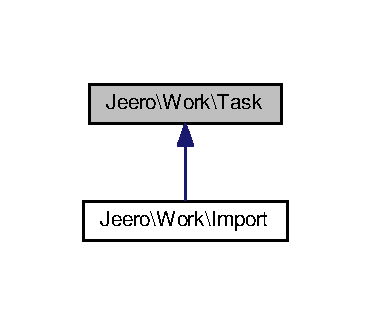
\includegraphics[width=178pt]{classJeero_1_1Work_1_1Task__inherit__graph}
\end{center}
\end{figure}


The documentation for this class was generated from the following file\+:\begin{DoxyCompactItemize}
\item 
Work/Task.\+php\end{DoxyCompactItemize}

\hypertarget{classJeero_1_1Calendars_1_1The__Events__Calendar}{}\section{Jeero\textbackslash{}Calendars\textbackslash{}The\+\_\+\+Events\+\_\+\+Calendar Class Reference}
\label{classJeero_1_1Calendars_1_1The__Events__Calendar}\index{Jeero\textbackslash{}\+Calendars\textbackslash{}\+The\+\_\+\+Events\+\_\+\+Calendar@{Jeero\textbackslash{}\+Calendars\textbackslash{}\+The\+\_\+\+Events\+\_\+\+Calendar}}


Inheritance diagram for Jeero\textbackslash{}Calendars\textbackslash{}The\+\_\+\+Events\+\_\+\+Calendar\+:\nopagebreak
\begin{figure}[H]
\begin{center}
\leavevmode
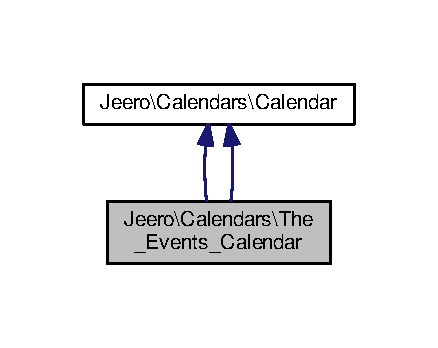
\includegraphics[width=210pt]{classJeero_1_1Calendars_1_1The__Events__Calendar__inherit__graph}
\end{center}
\end{figure}


Collaboration diagram for Jeero\textbackslash{}Calendars\textbackslash{}The\+\_\+\+Events\+\_\+\+Calendar\+:\nopagebreak
\begin{figure}[H]
\begin{center}
\leavevmode
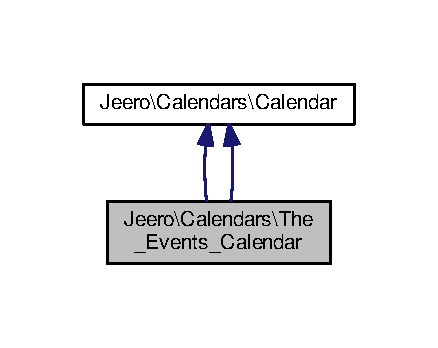
\includegraphics[width=210pt]{classJeero_1_1Calendars_1_1The__Events__Calendar__coll__graph}
\end{center}
\end{figure}


\subsection{Detailed Description}
\hyperlink{classJeero_1_1Calendars_1_1The__Events__Calendar}{The\+\_\+\+Events\+\_\+\+Calendar} class. 

The documentation for this class was generated from the following file\+:\begin{DoxyCompactItemize}
\item 
Calendars/The\+\_\+\+Events\+\_\+\+Calendar.\+php\end{DoxyCompactItemize}

\hypertarget{classJeero_1_1Theaters_1_1Theater}{}\section{Jeero\textbackslash{}Theaters\textbackslash{}Theater Class Reference}
\label{classJeero_1_1Theaters_1_1Theater}\index{Jeero\textbackslash{}\+Theaters\textbackslash{}\+Theater@{Jeero\textbackslash{}\+Theaters\textbackslash{}\+Theater}}


Inheritance diagram for Jeero\textbackslash{}Theaters\textbackslash{}Theater\+:\nopagebreak
\begin{figure}[H]
\begin{center}
\leavevmode
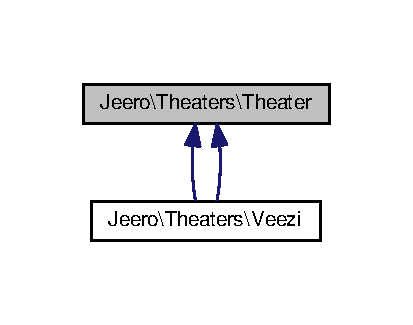
\includegraphics[width=198pt]{classJeero_1_1Theaters_1_1Theater__inherit__graph}
\end{center}
\end{figure}
\subsection*{Public Attributes}
\begin{DoxyCompactItemize}
\item 
\mbox{\Hypertarget{classJeero_1_1Theaters_1_1Theater_a1dd2ed0793c611738b97e74fa1f1f521}\label{classJeero_1_1Theaters_1_1Theater_a1dd2ed0793c611738b97e74fa1f1f521}} 
{\bfseries \$\+ID}
\end{DoxyCompactItemize}


\subsection{Detailed Description}
\hyperlink{classJeero_1_1Theaters_1_1Theater}{Theater} class. 

The documentation for this class was generated from the following file\+:\begin{DoxyCompactItemize}
\item 
Theaters/Theater.\+php\end{DoxyCompactItemize}

\hypertarget{classJeero_1_1Calendars_1_1Theater__For__WordPress}{}\section{Jeero\textbackslash{}Calendars\textbackslash{}Theater\+\_\+\+For\+\_\+\+Word\+Press Class Reference}
\label{classJeero_1_1Calendars_1_1Theater__For__WordPress}\index{Jeero\textbackslash{}\+Calendars\textbackslash{}\+Theater\+\_\+\+For\+\_\+\+Word\+Press@{Jeero\textbackslash{}\+Calendars\textbackslash{}\+Theater\+\_\+\+For\+\_\+\+Word\+Press}}


Inheritance diagram for Jeero\textbackslash{}Calendars\textbackslash{}Theater\+\_\+\+For\+\_\+\+Word\+Press\+:\nopagebreak
\begin{figure}[H]
\begin{center}
\leavevmode
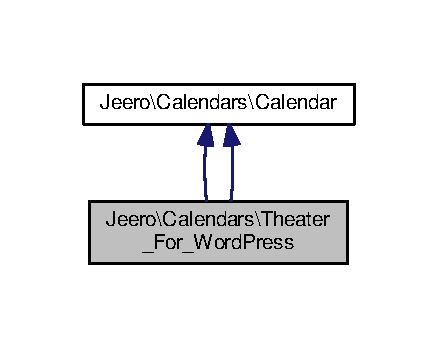
\includegraphics[width=210pt]{classJeero_1_1Calendars_1_1Theater__For__WordPress__inherit__graph}
\end{center}
\end{figure}


Collaboration diagram for Jeero\textbackslash{}Calendars\textbackslash{}Theater\+\_\+\+For\+\_\+\+Word\+Press\+:\nopagebreak
\begin{figure}[H]
\begin{center}
\leavevmode
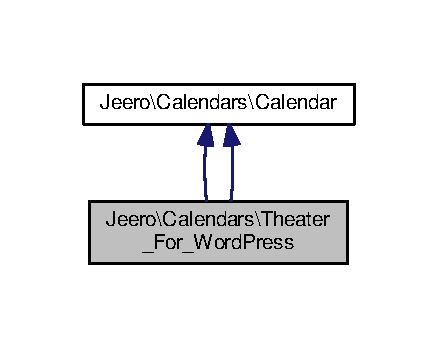
\includegraphics[width=210pt]{classJeero_1_1Calendars_1_1Theater__For__WordPress__coll__graph}
\end{center}
\end{figure}


\subsection{Detailed Description}
\hyperlink{classJeero_1_1Calendars_1_1Theater__For__WordPress}{Theater\+\_\+\+For\+\_\+\+Word\+Press} class. 

The documentation for this class was generated from the following file\+:\begin{DoxyCompactItemize}
\item 
Calendars/Theater\+\_\+\+For\+\_\+\+Word\+Press.\+php\end{DoxyCompactItemize}

\hypertarget{classJeero_1_1Theaters_1_1Veezi}{}\section{Jeero\textbackslash{}Theaters\textbackslash{}Veezi Class Reference}
\label{classJeero_1_1Theaters_1_1Veezi}\index{Jeero\textbackslash{}\+Theaters\textbackslash{}\+Veezi@{Jeero\textbackslash{}\+Theaters\textbackslash{}\+Veezi}}


Inheritance diagram for Jeero\textbackslash{}Theaters\textbackslash{}Veezi\+:\nopagebreak
\begin{figure}[H]
\begin{center}
\leavevmode
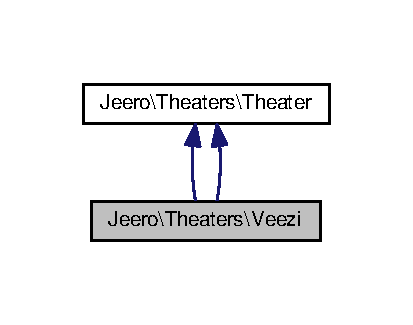
\includegraphics[width=198pt]{classJeero_1_1Theaters_1_1Veezi__inherit__graph}
\end{center}
\end{figure}


Collaboration diagram for Jeero\textbackslash{}Theaters\textbackslash{}Veezi\+:\nopagebreak
\begin{figure}[H]
\begin{center}
\leavevmode
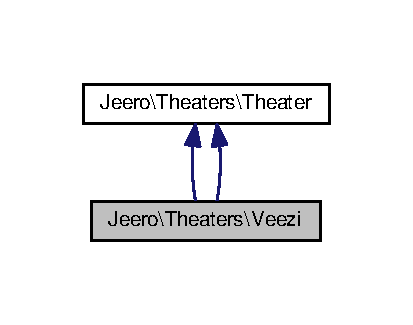
\includegraphics[width=198pt]{classJeero_1_1Theaters_1_1Veezi__coll__graph}
\end{center}
\end{figure}
\subsection*{Additional Inherited Members}


\subsection{Detailed Description}
\hyperlink{classJeero_1_1Theaters_1_1Veezi}{Veezi} class.

Handles the collection of films from \href{https://www.veezi.com/}{\tt Veezi} \hyperlink{namespaceJeero_1_1Theaters}{Theaters}.

\begin{DoxySince}{Since}
1.\+0 
\end{DoxySince}


The documentation for this class was generated from the following file\+:\begin{DoxyCompactItemize}
\item 
Theaters/Veezi.\+php\end{DoxyCompactItemize}

%--- End generated contents ---

% Index
\backmatter
\newpage
\phantomsection
\clearemptydoublepage
\addcontentsline{toc}{chapter}{Index}
\printindex

\end{document}
